\begin{figure}
	\centering
	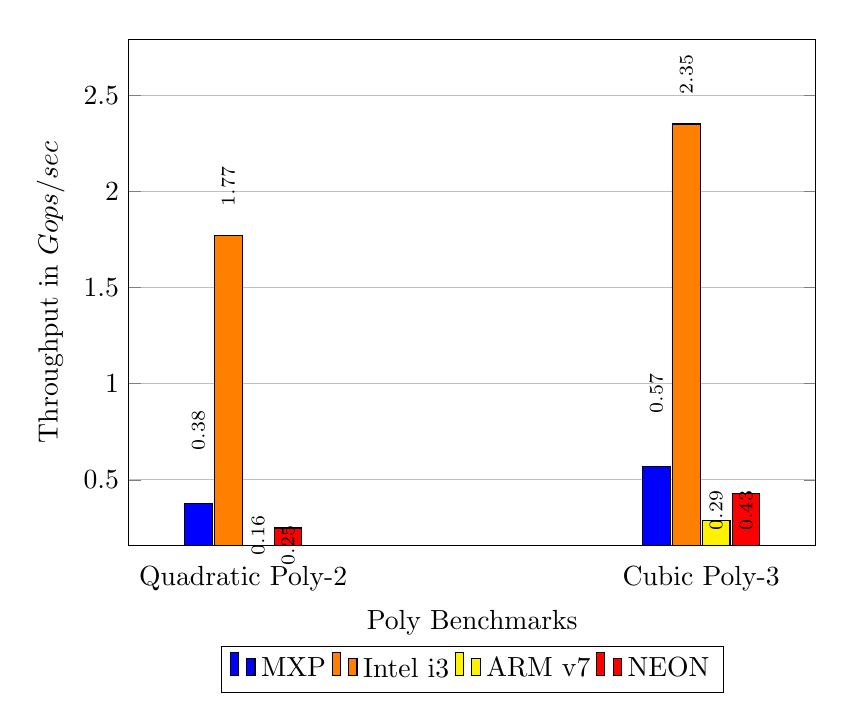
\begin{tikzpicture}
	\begin{axis}[
	width  = 0.85*\textwidth,
	height = 8cm,
	major x tick style = transparent,
	bar width=10pt,
	ymajorgrids = true,
	ylabel = {Throughput in $Gops/sec$},
	xlabel = {Poly Benchmarks},
	symbolic x coords={Quadratic Poly-2,Cubic Poly-3},
	xtick = data,
	nodes near coords,
	ybar,
	every node near coord/.append style={rotate=90, anchor=west,font=\scriptsize, xshift=0.25cm},
	scaled y ticks = false,
	enlarge y limits={upper,value=0.2},
	enlarge x limits=0.25,
	ybar=2*\pgflinewidth,
	legend cell align=left,
		legend style={
		at={(.5,-0.2)},
		anchor=north,
		legend columns=-1
		column sep=0.5ex
	}
	]
	\addplot[draw=black,fill=blue,every node near coord/.append style={xshift=0.3cm}]
	coordinates {(Quadratic Poly-2, 0.378) (Cubic Poly-3,0.571)};
	
	\addplot[draw=black,fill=orange]
	coordinates {(Quadratic Poly-2,1.77) (Cubic Poly-3,2.35)};
	
	\addplot[draw=black,fill=yellow,every node near coord/.append style={xshift=-0.50cm}]
	coordinates {(Quadratic Poly-2,0.1608) (Cubic Poly-3,0.2886)};
	
	\addplot[draw=black,fill=red,every node near coord/.append style={xshift=-0.85cm}]
	coordinates {(Quadratic Poly-2,0.2500) (Cubic Poly-3,0.4311)};
	
	\legend{MXP,Intel i3,ARM v7,NEON}
	\end{axis}
	\end{tikzpicture}
	\caption{Word(32-bits) level throughput(Gops/sec) for polynomial benchmarks }
	\label{poly:3}
\end{figure}
